Als we de Software\index{Software!Installatie} applicatie gestart hebben dan kunnen we
rechtsboven zoeken op een applicatie, we kunnen echter ook kiezen voor applicaties uit een Categorie. Klikken
we op Graphics \& Photography. Dan vinden we tussen de opties de GIMP\index{GIMP!Installatie}. Selecteer de GIMP en klik Install. Er zal
gevraagd worden om het root-wachtwoord, na dit ingevoerd te hebben begint de installatie.

Hierna kan je Software afsluiten of direct de GIMP opstarten.

\begin{figure}
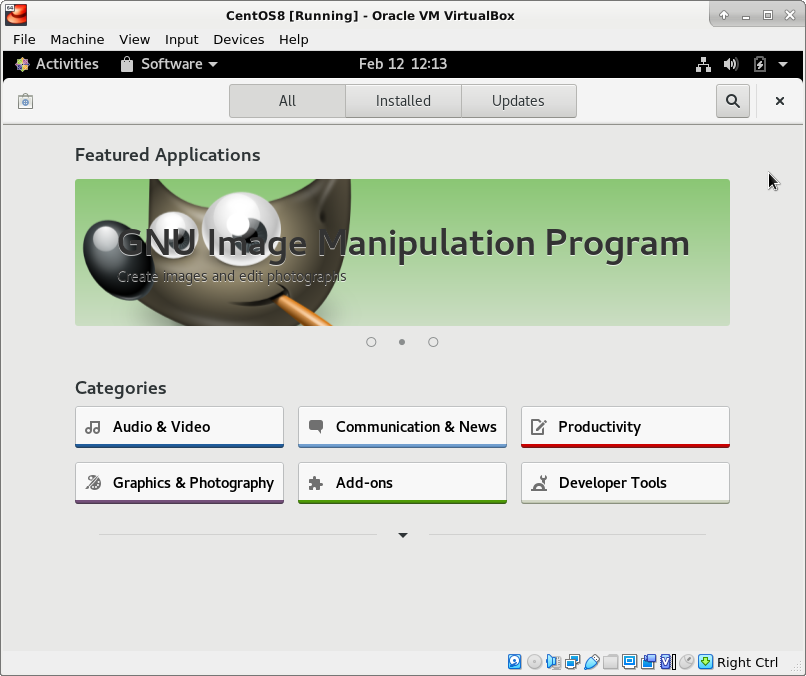
\includegraphics[width=0.9\textwidth]{linuxreader-img020.png}
	\caption{Ge\"installeerde GIMP}
	\label{fig:de_software_gimp}
\end{figure}
